\chapter{Background}\label{background}

In this chapter the reason for a documentation tool is outlined and some
existing solutions are described. Each existing solution will be analyses for
its strengths and weaknesses.

If code is written without comments or detail about what is to be
achieved then, it is possible that in the future, when the code is read again that the original intent is lost. The decisions the developer made about the implemented solution have been lost.

There are many different ways to document code they range from
completely offline to completely digital and many different methods for
integrating code. The most simple offline approaches consist of simple
notepad pages with notes and diagrams. This offers a totally freeform
approach to note taking as with pen and paper there is no limit to what
you can make notes about. Tables diagrams and hand written pseudo code
can be easily drawn and annotated. While this is suitable for some circumstances it isn't for others. For example if you had an email you wanted to include in your notes it would have to be printed and filed in the notes. This leads to problems of printing and loosing loose pages.

One solution for this problem is the many solutions for electronic or digital
notes. \textit{Evernote}\cite{evernote} is a popular choice for notes and offers
a wide range of platforms for note creation however it is not designed with code
documentation in mind specifically. While it is a very good solution for taking
notes as is evident in the number of users\footnote{The current raking of
Evernote by Alexa is 397
\href{http://www.alexa.com/siteinfo/evernote.com}{http://www.alexa.com/siteinfo/evernote.com}}.
the lack of specific features aimed at developers for example, version control.
This makes it difficult to use in this way.

The above solutions are not tailored to suit the specific task of making notes
for sql developers. Tools used by developers can both develop new code and help
document it for future readers. Commenting code is often the closest notes get
to the code. Well commented code can help developers to both remember the code
they wrote in the past and understand new code. Comments provide an excellent
opportunity to pass details of previous attempts from programmer to programmer.

Comments on code can often not last the test of time as they don't force you to
update your note when the code they refer to changes. For example, over time the
commented function might offer more options or deviate from its original
purpose. Unless the developer remembers to update the comment then, over time, this could lead to confusion.

\section{Analysis of existing solutions}\label{analysis-of-existing-solutions}

The different applications vary from exact programming language and
operating system. They each have positives and negatives.

Each is analyzed below with a brief overview of the functionality provided and details on specific positives and negatives. After the analysis of the existing solutions the problems will be summarized before requirements are set out.


\begin{figure}
  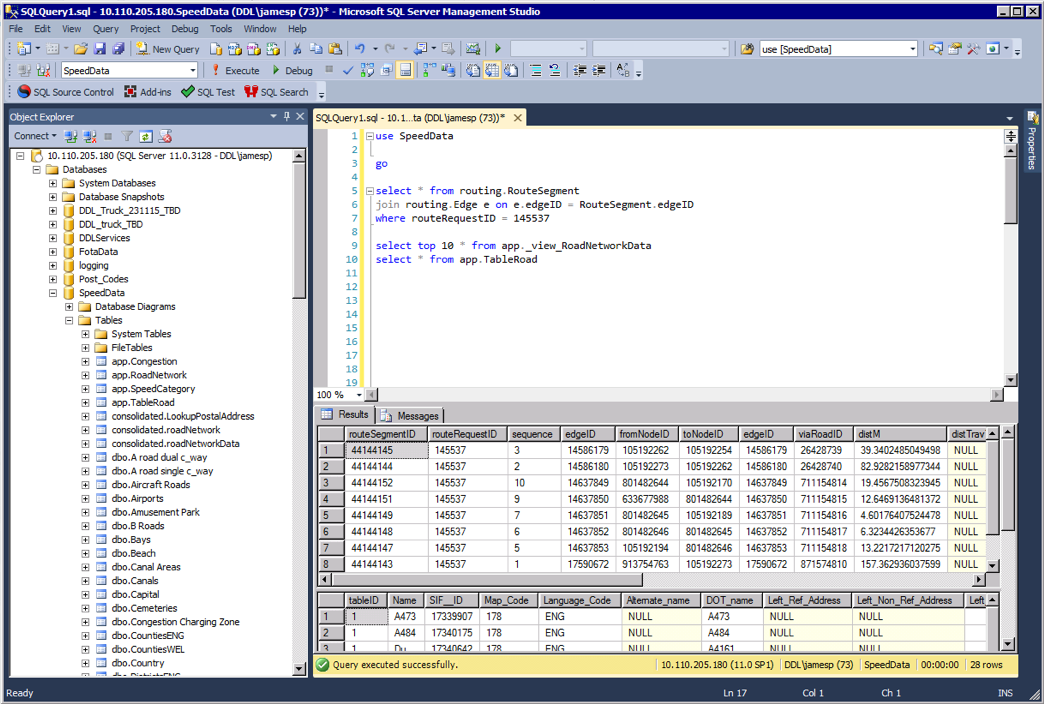
\includegraphics[width=\linewidth]{Figures/SSMS.png}
  \caption{SQL Server Management Studio, Microsoft: Main workspace with open queries and results}
  \label{fig:ssms}
\end{figure}

\subsection{Microsoft SQL Server Management Studio}\label{microsoft-sql-server-management-studio}

\noindent
See fig \ref{fig:ssms} for a screenshot.

\noindent

\textbf{Product URL}\cite{ssms}
\url{https://msdn.microsoft.com/en-us/library/hh213248.aspx}



An official offering for the Microsoft SQL Server Database server. The ability
to open multiple connections to databases and have many open files in an IDE
powered with the Microsoft Visual Studio Shell\cite{vsshell}. The application
offers no management of files within the tool, it does however, offer the
ability to open files from the filesystem. The tool allows for the execution of queries and the result viewing pane shows a table containing the output. The results in the result pane can not be stored in the application or with the query for later review if this is a requirement of a user it must be done manually with the export function.

As with many database servers the functions and procedures are stored within the
databases and so any files on the local system might not be in sync with the
ones on the server. The application is a native windows application and offers
no alternatives for other operating systems. Developers have the ability to
connect via TCP, Shared memory, and named pipes. This allows for connections to be made from anywhere with a suitably open internet connection however it poses many problems when on a restricted network and limits users to use Microsoft's
own operating system as the application is for Windows only.

\blockquote{Windows 10, Windows 8, Windows 8.1, Windows 7 (SP1), Windows Server 2012 (64-bit), Windows Server 2012 R2 (64-bit), Windows Server 2008 R2 (64-bit)}

From SSMS 2016 preview download page \cite{ssmsdownload}.


\begin{figure}
  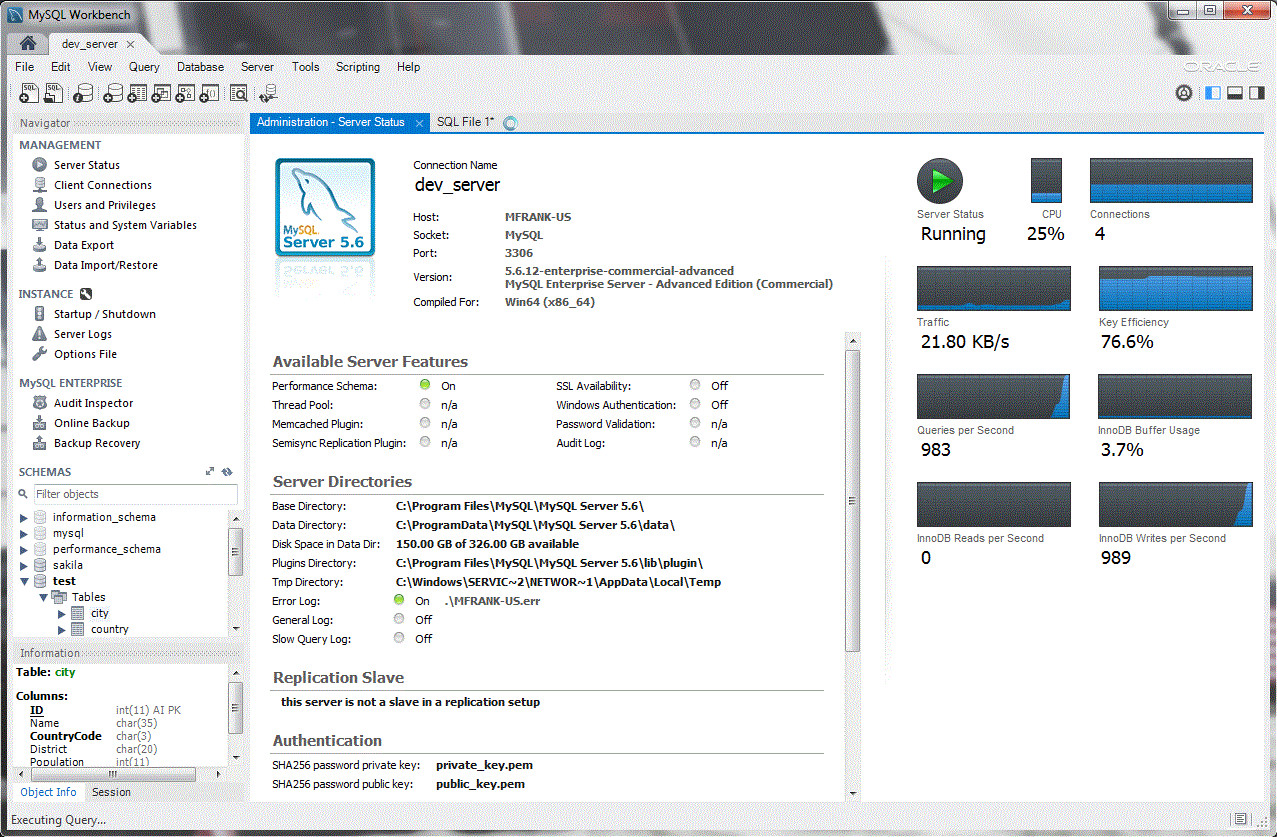
\includegraphics[width=\linewidth]{Figures/MySqlWorkbench.png}
  \caption{MySql Workbench, Oracle: Home screen}
  \label{fig:mysqlworkbench}
\end{figure}

\subsection{MySQL Workbench}\label{mysql-workbench}

\noindent
See fig \ref{fig:mysqlworkbench} for a screenshot.

\noindent
\textbf{Product URL}\cite{mysqlworkbench}
\url{https://www.mysql.com/products/workbench/}


The MySQL Workbench offers a multi-platform solution for accessing a
MySql database. The tool also offers a model management tool (fig \ref{fig:mysqlworkbenchmodel}) for designing
a logical model of the database entities and relations, this provides a way to
easily view a high level overview and make useful annotations that go
above and beyond simple comments written separately. For more information Oracle have published a paper detailing the creation of the tool\cite{mysqlworkbenchmodeldesign}.

\begin{figure}
  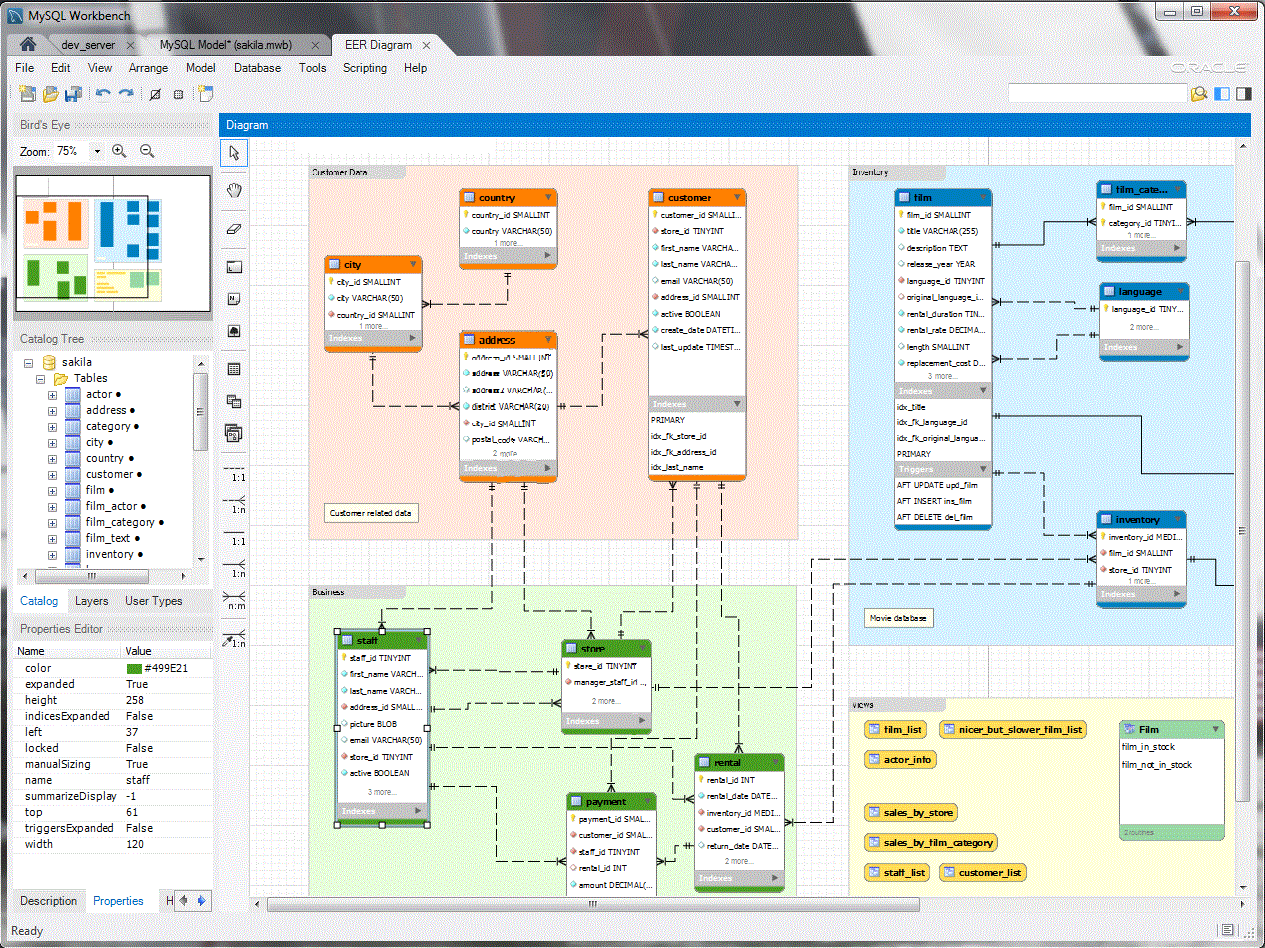
\includegraphics[width=\linewidth]{Figures/MySqlWorkbenchModel.png}
  \caption{MySql Workbench, Oracle: Visual Database Design feature}
  \label{fig:mysqlworkbenchmodel}
\end{figure}

The Workbench also offers multi-platform capability. Providing more ways for the
users of an application helps integrate a tool into the workflow of the
developer, having to switch between operating systems because your database
management software is not offered on the same work machine as your front end
development environment. Applications that are not cross-platform pose a problem to the users who develop on another platform the development of this project should aim to support common platforms.


\begin{figure}
  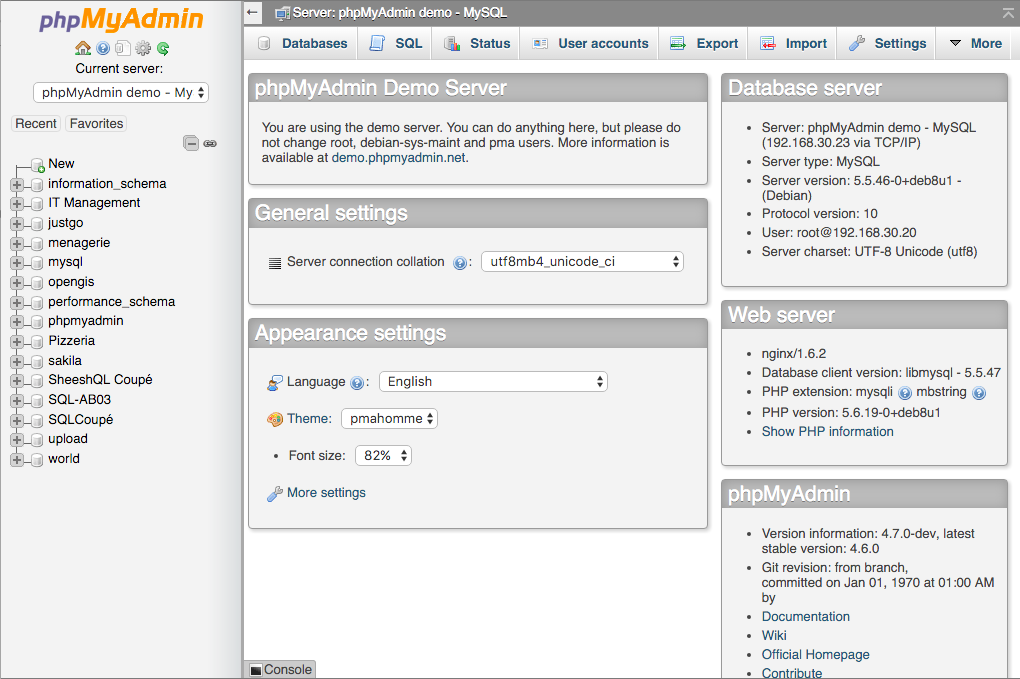
\includegraphics[width=\linewidth]{Figures/phpmyadmin.png}
  \caption{phpMyAdmin: home page}
  \label{fig:phpmyadmin}
\end{figure}


\subsection{phpMyAdmin}\label{phpmyadmin}

\noindent
See fig \ref{fig:phpmyadmin} for a screenshot.

\noindent
\textbf{Product URL}\cite{phpmyadmin}
\url{https://www.phpmyadmin.net/}


The alternative to the official MySqlWorkbench is an open source web
based solution for easy access to the database from anywhere you have an
internet connection. phpMyAdmin is a PHP web application and needs a
hosting server to provide access. The application, once running
has a secure login system with the ability to view and edit data in the
system.

However the tool offers little in the way of editing for scripts and
database code. Bulk manipulation of data is not offered in the
application but instead through the export of multiple different file
types.

The application also analyses the foreign keys in the database and provides access to the referenced rows in the related tables. This feature can make viewing the data in the system more intuitive as related data need not be separately queried for.

Unlike the MySql Workbench there is no designer for models and all
changes are done to the database ``live'' there is no design and publish
as offered in MySql workbench.


\begin{figure}
  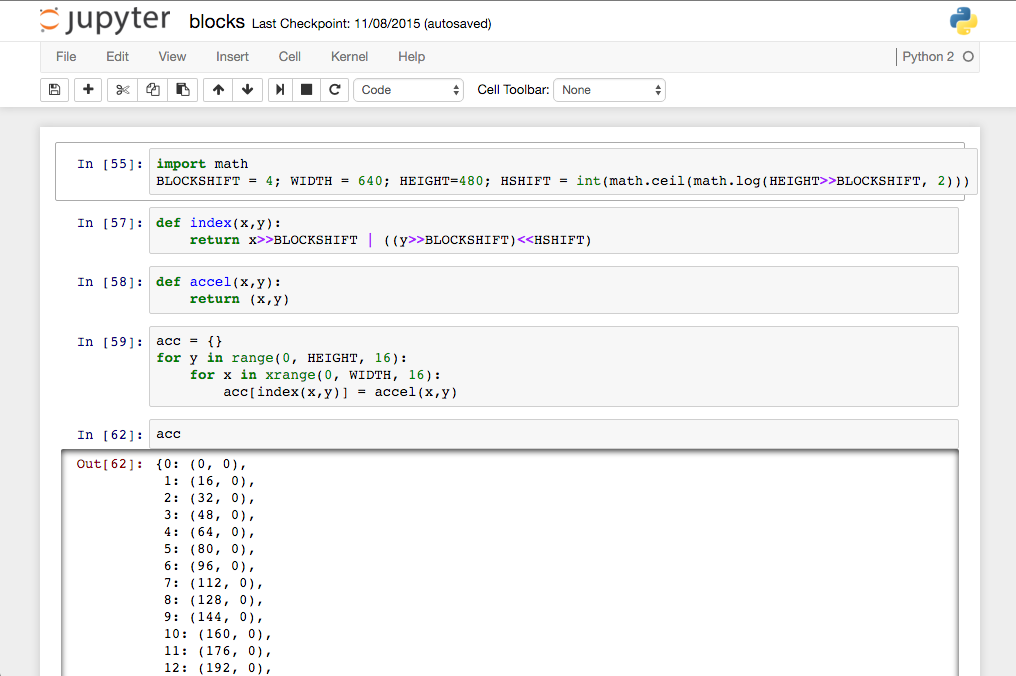
\includegraphics[width=\linewidth]{Figures/ipython.png}
  \caption{IPython Notebook, example notebook}
  \label{fig:ipythonnotebook}
\end{figure}

\subsection{IPython / Jupyter}\label{ipython-jupyter}

\noindent
See fig \ref{fig:ipythonnotebook} for a screenshot.

\noindent
\textbf{Product URL}\cite{PER-GRA:2007}
\url{http://ipython.org/}

IPython, now Jupyter, differs from other solutions evaluated above as it is not
a SQL IDE and such it doesn't show any specific features for SQL code in
particular however the integration between the code and the text in the editor
is done in a very easy to use way.

IPython provides an interactive browser based coding tool the ``notebook''. The notebook provides the ability to create cells for code and text. The code can be executed and results are shown below the code. The text cells are formatted with Markdown\cite{wiki:markdown}.

\begin{figure}
  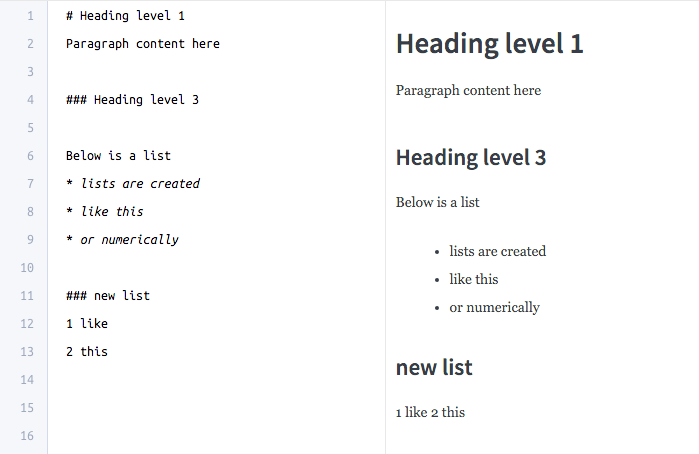
\includegraphics[width=\linewidth]{Figures/markdown.png}
  \caption{Markdown: example markdown source (left) and output (right)}
  \label{fig:markdownexample}
\end{figure}

Markdown (fig \ref{fig:markdownexample}) is a simple written markup language for
textual documents. Markdown provides simple ways to create headings and lists
paragraphs while balancing this with simple easy to read minimal formatting.

The mix of executable code within the text notes provides a unique
experience. The ability to see and tweak code and have a well
presented explanation of the code.

Interactive code and results as done in an IPython notebook provide a
quick way to see the results of the code. This allows and promotes the
testing and exploration of the code and can help the developer to
understand exactly what effects each part of the code has on the end
result. This is important because developers who understand the impact of the existing code and their changes to it will create less bugs in code and are more productive.

The notebooks reside on files on the local disk of the system, much like
any other file. As such the organization of the files is left up to you
the creator to file them in folders etc. This can be a problem for long term users of the application as while the individual files might be organized, if the collection of files is haphazard then the organization problem has just moved to another part of the process.

\section{Problems}\label{problems}

\begin{problem}{Keeping notes of important things}

As developers work on their projects and as these projects evolve there
become an increasing number of things that need to be understood in
order to develop / maintain the project. The problem is to provide an
easy flexible way to make notes on different topics and allow access to
the notes in an organized way.

\end{problem}

\begin{problem}{Notes are only useful when they are read}

The notes / code stored need to be accessible for developers, they are read more times than they are modified. This shows the importance of the time spend documenting the code when it is first written.

The notes as discussed do not have an implicit structure and so a helpful
search is difficult to create. Most solutions just offer full text
search of the data.

The notes might have had several revisions over time and might need the
information accessible from the past.

\end{problem}


\begin{problem}{Notes that include code are often not
updated}

The notes, in some note taking applications that store code, are often not in an
executable format. This code will have dependences as code does not exist in isolation. For example the functions used or the tables referenced may be modified. If the code in the note can not be directly executed, these changed in the context can create bugs in the code that wont be immediately visible and could mislead the reader.

This is a problem because the code is only useful in a note when it is
up to date and bug free, often at the time of writing it is correct but
as the system changes the code can become out of date.

The problem is how to ensure or help the user to keep this code up to
date within the note.

\end{problem}

\begin{problem}{Data always changing}

The data in database systems is always changing, when the system was
written the data might have looked significantly different to what it is
now. This makes things hard to compare as time goes on.

The problem is how to ensure that, even if the underlying data is
changed, the note and code within is still useful for other developers
in the future.

\end{problem}

\begin{problem}{System access}

Developers need easy access to the information and the database from in or out of the office. Current solutions for IDE's are often system specific and
don't offer good cross platform compatibility.

The problem is providing access to the data and system from whatever
system, and wherever the developer is in a secure way.
\end{problem}

\begin{problem}{Cross referencing}

When writing documents, often it is required to provide context. This is done by referring to other parts of the same or different document. Providing a solution to this problem will benefit both the readers and writers and help communicate the information.

\end{problem}

\section{Problem summary}\label{summary-of-identified-problems}

The problems identified above fall into different categories:

\begin{itemize}
\tightlist
\item
  Organization of notes
\item
  SQL specific problems
\item
  Searching notes
\end{itemize}

Each of the above categories of problems could be tackled in many different
ways. The next stage in the development of a complete solution is to identify
some concrete requirements and use cases for the application and discuss the
different approaches available. Each approach has downsides, these need to be
properly analyzed and evaluated to provide a solution.
